\documentclass[tikz,border=2pt]{standalone}

\usepackage{tikz}
\usetikzlibrary{positioning}

\begin{document}

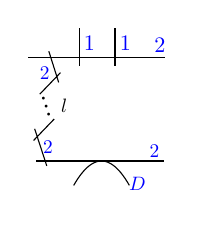
\begin{tikzpicture}[xscale=0.57,yscale=0.62]

% Long horizontal 2-component, meeting the lower end of the first
% diagonal component of the zigzag.
\draw (1.85,-0.12) -- (4.70,-0.12);
\node[blue,scale=0.7,above] at (4.48,-0.18) {$2$};

% Small D-component, drawn as a frown and tangent to the horizontal
% 2-component.
\draw[domain=-0.62:0.62,samples=80,smooth,variable=\t]
  plot ({3.30+\t},{-0.12-1.3*\t*\t});
\node[blue,scale=0.7] at (4.1,-0.58) {$D$};

% Zigzag. The first diagonal component has the usual chain-component length.
\draw (2,0)

++(0.08,-0.22)
--++(-0.27,0.76)
node[midway,blue,scale=0.7,right,inner sep=1pt] {$2$}
++(0.135,-0.26)


++(0,0.02)
++(0,-0.02)

++(-0.16,0.02)--++(0.46,0.44)++(-0.12,0.08)

node {$\cdot$} ++(-0.06,0.16) node {$\cdot$}
++(-0.06,0.16) node {$\cdot$} ++(0.17,-0.12)
node[auto,inner sep=5,scale=0.7,anchor=west] {$l$}

++(-0.25,0.23)--++(0.46,0.44)++(-0.19,0.04)

++(0,-0.05)
node[blue,scale=0.7,inner sep=1,anchor=east] {$2$}

++(0,0.05)
++(0.19,-0.04)++(-0.04,-0.2)--++(-0.22,0.64);

% Top tail component.
\draw[shorten >=2] (5/3,2)--(29/6,2)
  node[inner sep=2pt,blue,above left,scale=0.8] {$2$};

\draw[shorten <=-3pt] (14/5,2)
  -- node[inner sep=2pt,scale=0.8,blue,right] {$1$}
  (14/5,13/5);

\draw[shorten <=-3pt] (18/5,2)
  -- node[inner sep=2pt,scale=0.8,blue,right] {$1$}
  (18/5,13/5);

\end{tikzpicture}

\end{document}

